% !TeX spellcheck = fr_FR
% !TeX encoding = ISO-8859-1

\section{L'effet}

Le � bon effet � prolonge le mouvement de la bille, l' � effet contraire
� ralentit le mouvement de la bille, voir \autoref{fig:a04-1}. L'effet ne produit son effet qu'en rencontrant un obstacle.
Les changements de direction dus � l'effet seront d'autant plus
importants qu'on jouera bas de bille.

Fig l : L'effet est contraire sur la bille 2 et bon sur la bande : la
1 aura tendance � s'�tendre le long de la bande donc � s'�carter de la
perpendiculaire au point d'impact sur la bande, ou, si l'on pr�f�re :
l'angle de r�flexion sera plus grand que l'angle d'incidence.

Fig 3: L'effet est bon sur la bille 2 et contraire sur la bande. La 1 aura tendance � retenir son mouvement donc � se rapprocher de la
perpendiculaire � la bande au point d'impact : l'angle r�fl�chi sera
plus petit que l'angle d'incidence.

Fig 2 : Cette figure montre le ph�nom�ne d'engrenage de l'effet. Tout se passe comme si les billes �taient des roues dent�es. Quand la 1
rencontre la deux, elle lui donne une partie de son �nergie sous forme
de rotation dont le sens sera inverse � celui d'origine ... comme avec
les engrenages. 
\begin{itemize}
\item Ainsi, si nous imprimons � la 1 une rotation gauche, au moment de l'impact avec
la 2, elle imprimera � celle-ci une rotation droite. L'effet de la 2
sera plus faible que celui d'origine mais pas du tout inexistant. On
constatera le ph�nom�ne de deux fa�ons : la 2 est l�g�rement d�vi�e dans
le sens de l'effet de la 1 et au toucher de la premi�re bande, elle aura
une d�viation correspondant � l'effet inverse de la 1.
\item C'est en � soutenant � bien son � coup � qu'on imprimera une
part plus importante d'effet � la 2. Ce ph�nom�ne d'engrenage est
capital pour rappeler des positions qui sans cela, seraient perdues. La
bonne compr�hension de ce ph�nom�ne facilitera grandement l'�tude du jeu
de rappel.
\end{itemize}

\begin{figure}[htb]
	\centering
	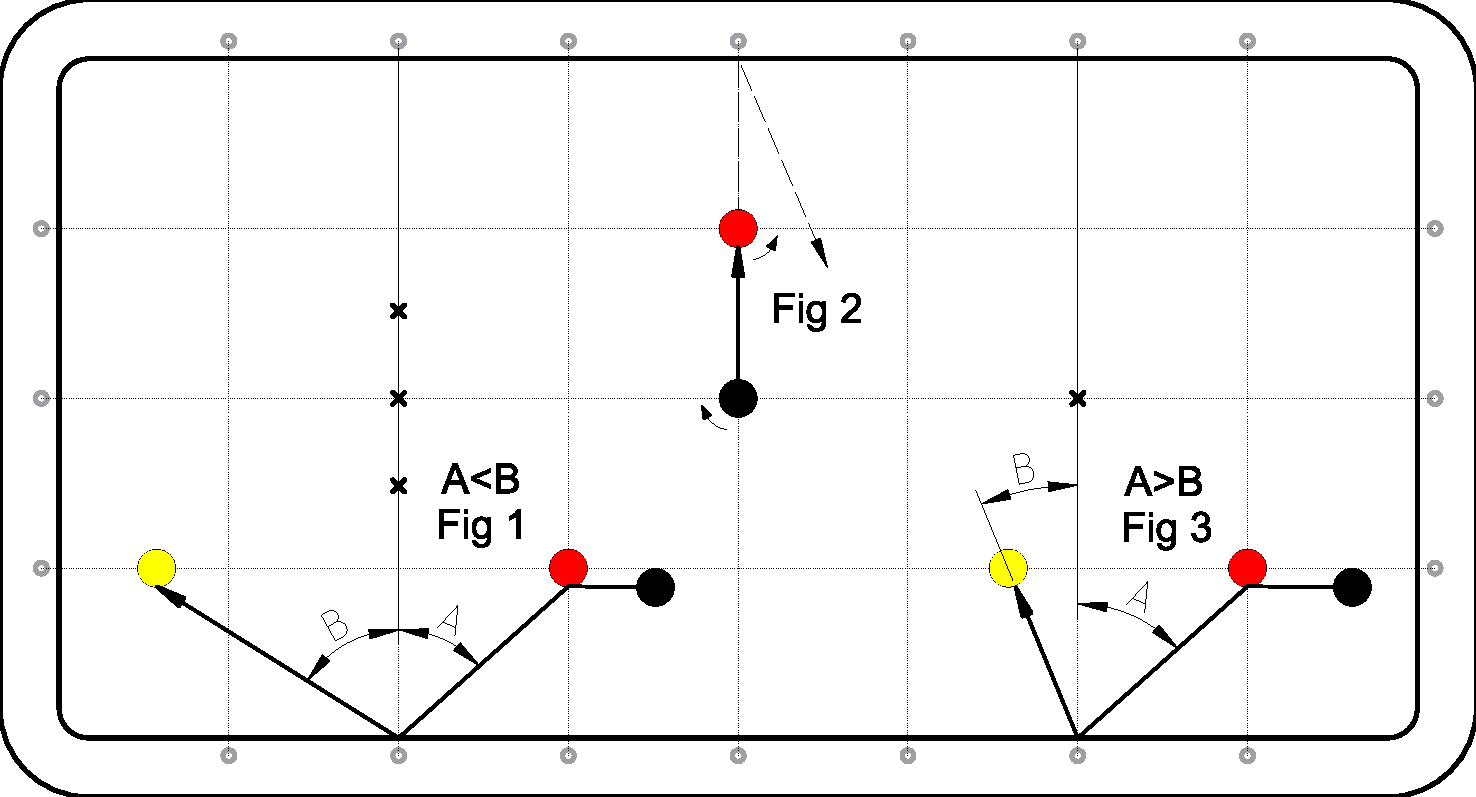
\includegraphics[width=\linewidth]{A/imagesA/A04-1.pdf}
	\caption{Effet contraire, engrenage et bon effet.}
	\label{fig:a04-1}
\end{figure}

\clearpage